\begin{sol}
\begin{enumerate}[label=\textbf{(\alph*)}]
\item
$$-\frac{1}{2m}\frac{d^2\psi}{dx^2}+(\alpha x^4-E)\psi=0$$
Let $x=\beta u$
$$-\frac{1}{2m}\frac{d^2\psi}{du^2}\Big(\frac{du}{dx}\Big) ^2+(\alpha \beta^4u^4-E)\psi=0$$
$$-\frac{1}{2m\beta^2}\frac{d^2\psi}{du^2}+(\alpha\beta^4u^4-E)\psi=0$$
Let $e=\frac{E}{\alpha\beta^4}$ 
$$-\frac{1}{2m\alpha\beta^6}\frac{d^2\psi}{du^2}+(u^4-e)\psi=0$$
$$-\frac{1}{2}\frac{d^2\psi}{du^2}+(u^4-e)\psi=0$$
It is found that $m\alpha\beta^6=1$ and $E=\alpha\beta^4e$. For convenience, define a reduced Hamiltonian
$$\hat h=\frac{1}{\alpha\beta^4}\hat H$$

\item
$e=0.667986$ \\
\begin{center}
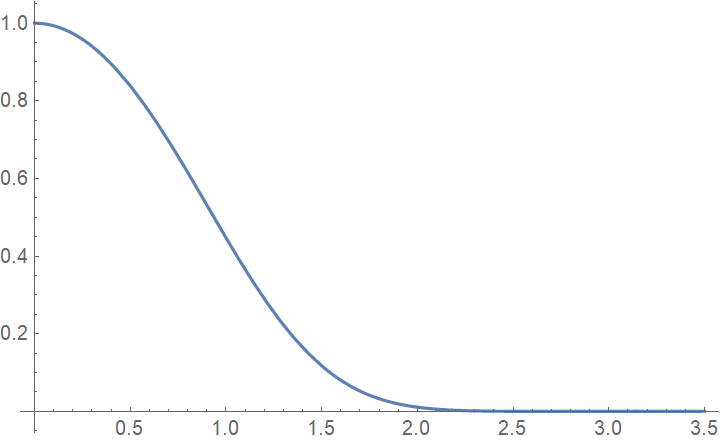
\includegraphics[scale=0.4]{P02/HO4.png}
\end{center}
\item
It appears that this wave-function looks like a gaussian, which is known to be the ground state of the simple harmonic oscillator potential. Thus, a good candidate wavefunction for the first excited state of this potential is the first excited state of the simple harmonic oscillator, 
$$\braket{x}{\psi_\alpha}=u\exp(-\alpha u^2)\text{ where }\alpha>0, \alpha\in\mathbb R$$ 
Where $u\equiv\frac{x}{\beta}$. Show that all states $\ket{\psi_\alpha}$ are all orthogonal to the ground state
$$\braket{0}{\psi_a}=\int_{-\infty}^\infty\braket{0}{u}\braket{u}{\psi_a}dx=\int_{-\infty}^\infty\braket{0}{u}u\exp(-\alpha u^2)dx$$ 
Note the ground state is even
$$\braket{0}{\psi_a}=\int_0^\infty\braket{0}{u}u\exp(-\alpha u^2)du+\int_{-\infty}^0\braket{0}{u}u\exp(-\alpha u^2)du$$
For the second term, let $k=-u$ then $dk=-du,u=-k,\braket{0}{k}=\braket{0}{x}, u^2=k^2$.
$$\braket{0}{\psi_a}=\int_0^\infty\braket{0}{u}u\exp(-\alpha u^2)du+\int_{\infty}^0\braket{0}{k}k\exp(-\alpha k^2)dk$$ 
Re-substituting $u=k$.
$$\braket{0}{\psi_a}=\int_0^\infty\braket{0}{u}u\exp(-\alpha u^2)du-\int_{0}^\infty\braket{0}{u}u\exp(-\alpha u^2)du=0$$
Therefore, the variational principle can be applied to obtain a upper bound on the first excited state
$$e_1\leq\frac{\bra{\psi_a}\hat h\ket{\psi_a}}{\braket{\psi_a}{\psi_a}}=\frac{2^\frac{5}{2}\alpha^\frac{3}{2}}{\sqrt\pi}\int_{-\infty}^\infty u\exp(-\alpha u^2)\left(-\frac{1}{2}\frac{d^2}{du^2}+u^4\right)\left(u\exp(-\alpha u^2)\right)$$  
$$=\frac{2^\frac{5}{2}\alpha^\frac{3}{2}}{\sqrt\pi}\int_{-\infty}^\infty \exp(-2\alpha u^2)\left(u^6-2a^2u^4+3au^2\right)du=\frac{2^\frac{5}{2}\alpha^\frac{3}{2}}{\sqrt{\pi}}\frac{3\sqrt{\pi}(5+8\alpha^3)}{2^\frac{13}{2}\alpha^\frac{7}{2}}=\frac{3}{16}(5\alpha^{-2}+8\alpha)$$ 
It is easy to see that the bound is concave for $\alpha>0$, thus, the stationary point will be the minimum point. Taking the derivative with respect to $\alpha$ yields
$$\frac{3}{16}(-10\alpha^{-3}+8)=0$$
$$10=8\alpha^3\text{ so }\alpha=\frac{10^{\frac{1}{3}}}{2}\approx 1.07722\text{ and }\alpha^{-2}\approx 0.861774$$   
The upper bound can be calculated to be $e_1\leq 2.423$.
\newpage
\item
The next lowest value of $e$ is about $2.394$. The wave function looks like this\\
\begin{center}
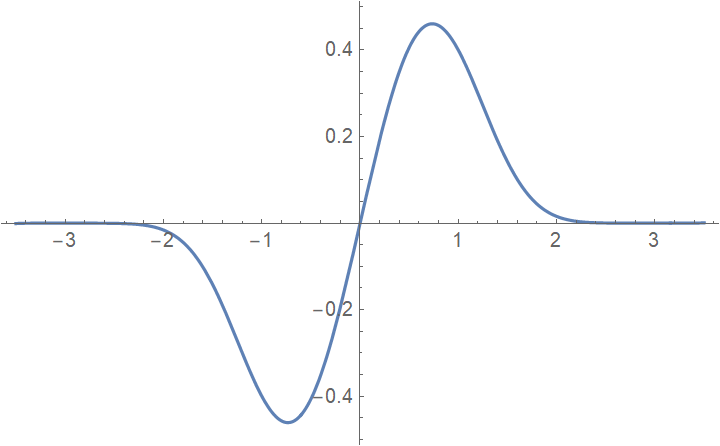
\includegraphics[scale=0.4]{P02/HO1.png}
\end{center}
\end{enumerate}
\end{sol}